\documentclass[10pt]{beamer}

\usepackage[utf8]{inputenc}
\usepackage[T1]{fontenc}
\usepackage{amsmath,amssymb,amstext}
\usepackage{mathrsfs}
\usepackage{siunitx}
\usepackage{multimedia}
\usepackage{nccfoots}

\usepackage{scrextend}
\changefontsizes{7pt}

\usepackage{array}
\newcolumntype{P}[1]{>{\centering}p{#1}}

\usepackage{overpic}

\usepackage{ufcd}
\usepackage[english]{babel}
\usepackage[backend=biber,backref=false,style=numeric-comp, sorting=none,block=ragged,firstinits=true]{biblatex}

\addbibresource{fp_refs.bib}

\usetheme{ufcd}

\newcommand{\gra}[3][]{
	\begin{table}
	\centering
	\begin{tabular}[width=\textwidth]{c}
		\includegraphics[width=#1\textwidth]{../figures/#2.png}\\
		\small #3
	\end{tabular}
	\end{table}
}
\newcommand{\graTwo}[5][]{
	\begin{table}
		\centering
		\begin{tabular}[width=\textwidth]{cc}
			\includegraphics[width=#1\textwidth]{../figures/#2.png}&
			\includegraphics[width=#1\textwidth]{../figures/#3.png}\\
			\small #4&\small #5
		\end{tabular}
	\end{table}
}
\newcommand{\graThree}[6][0.49]{
	\begin{tabular}[width=\textwidth]{ccc}
		\includegraphics[width=#1\textwidth]{../figures/#2.png}&
		\includegraphics[width=#1\textwidth]{../figures/#3.png}&
		\includegraphics[width=#1\textwidth]{../figures/#4.png}&
		\captionof{figure}[#5]{#6}
	\end{tabular}
}	
\newcommand{\graFour}[9][]{
	\begin{tabular}[width=\textwidth]{cc}
		\includegraphics[width=#1\textwidth]{../figures/#2.png}&
		\includegraphics[width=#1\textwidth]{../figures/#3.png}\\
		\small #6&\small #7\\
		\includegraphics[width=#1\textwidth]{../figures/#4.png}&
		\includegraphics[width=#1\textwidth]{../figures/#5.png}\\
		\small #8&\small #9
	\end{tabular}
	}
\newcommand{\graTwoOne}[4][]{
	\begin{table}
		\centering
	\begin{tabular}[width=\textwidth]{cc}
		\includegraphics[width=#1\textwidth]{../figures/#2.png}&
		\includegraphics[width=#1\textwidth]{../figures/#3.png}
	\end{tabular}
	{#4}
	\end{table}
}
\newcommand{\graTwoOneB}[4][]{
	\begin{table}
		\centering
		\begin{tabular}[width=\textwidth]{c}
			\includegraphics[width=#1\textwidth]{../figures/#2.png}\\
			\includegraphics[width=#1\textwidth]{../figures/#3.png}\\
			#4
		\end{tabular}
	\end{table}
}
\newcommand{\graTwoOneC}[5]{
	\begin{table}
		\centering
		\begin{tabular}[width=\textwidth]{cc}
			\includegraphics[width=#1\textwidth]{../figures/#3.png}&
			\includegraphics[width=#2\textwidth]{../figures/#4.png}\\
		\end{tabular}
		#5
	\end{table}
}
\newcommand{\nlOne}{\\&\small }
\newcommand{\nlTwo}{\\&\small }
\newcommand{\degree}{^\circ}

%\setbeamerfont{footnote}{size=\tiny}



\title{Holography}
\author{Saskia Bondza \& Simon Stephan}
\date{04.04.2017}

\begin{document}
\maketitle
\frame{\tableofcontents}
\section{Theoretical Background}
\frame{\tableofcontents[currentsection]}
\begin{frame}
	\frametitle{Holography - What is it?}
	\gra[0.35]{holo-schach}{}
	\Footnotetext{}{http://www.holoworld.com/holo/images/hologram.jpg}
		\begin{tabular}{p{5cm}|p{5cm}}
			\textbf{Photography}&\textbf{Holography}\\\hline
			2-dimensional images&3-dimensional images\\\hline
			stores only amplitude information&stores amplitude and phase information\\\hline
			can be seen at any light&can be seen only with the same beam as recorded with
		\end{tabular}
\end{frame}

\begin{frame}
	\frametitle{Princple Set-Up of a Holography experiment}
	\gra[0.8]{PrincipleSetUp}{}
	Functioning Principle: Interference on the Photographic plate $\rightarrow$ Coherent light source as condition
	\footnotetext{By DrBob at the English language Wikipedia, CC BY-SA 3.0, https://commons.wikimedia.org/w/index.php?curid=18103931}
\end{frame}

\begin{frame}
	\frametitle{Interference}
	\begin{table}
		\centering
		\begin{tabular}[width=\textwidth]{m{6cm}m{4cm}}

				
			\gra[0.6]{stripes}{Interference Pattern of two Plane Waves\footnote{http://www.mdpi.com/2072-666X/2/2/221/htm}}
			&
			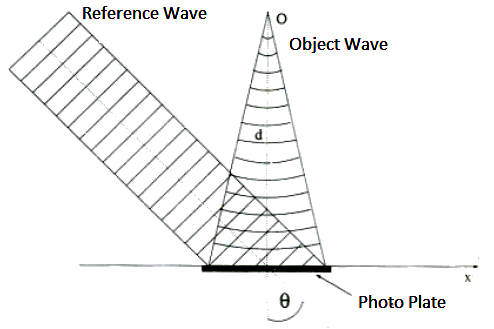
\includegraphics[width=0.4\textwidth]{../figures/Interference1.png}\newline
			{\small Interference on the photographic plate\footfullcite{staats}}\\
		\end{tabular}
		\begin{align*}
		A_1(r) &= E_1(r) e^{i(kr+\phi_1)}\\
		A_2(r) &= E_2 e^{i(kx\sin(\theta)+\phi_2)}\\
		I&=I_1+I_2+2\sqrt{I_1I_2}\cos(k(r-x\sin\theta))
		\end{align*}
	\end{table}
	%\Footnotetext{2}{\fullcite{staats}}
\end{frame}


\begin{frame}
	\frametitle{Hologram of an object point}
	\begin{tabular}{m{5cm}m{5cm}}
	\graTwoOneB[0.2]{obj1}{obj1b}{}
	Blackness of a photo plate for an object point\newline(spherical wave) \footfullcite{staats}\pause&
	\gra[0.5]{Reconstruction1}{Reconstruction of the Hologram \footnotemark[3]}
	\end{tabular}\pause
	$A(r)=\underbrace{[T_0-Ct_B(I_1+I_2)]A_R\ e^{ikx \sin\theta}}_{\mbox{no information}} - \underbrace{\sqrt{I_1I_2}A_RCt_B\ e^{ikr}}_{\mbox{virtual image}} - \underbrace{\sqrt{I_1I_2}A_RCt_B\ e^{-ikr}e^{2ikx \sin\theta}}_{\mbox{real image}}$
	
\end{frame}
\begin{frame}
	\frametitle{Coherence}
	\textbf{Coherence:} Degree of correlation of physical quantities of a single wave or between multiple waves or even wave packets
	
	Added up Intensity of coherent Waves:
	
	\begin{align*}
	I=\left| a_1 e^{i \phi_1} + a_2 e^{i \phi_2} \right|^2 = \left(I_1+I_2 \right) \left[ 1 + m \cos(\Delta \delta)\right], 
	\end{align*}
	
	Added up Intensity of incoherent waves:
	
	\begin{align*}
	I=\left| a_1 e^{i \phi_1} \right|^2+ \left| a_2 e^{i \phi_2}\right|^2 = I_1+I_2
	\end{align*}

	\begin{table}
		\centering
		\begin{tabular}{m{5cm}m{5cm}}
			\textbf{Temporal Coherence}&\\
			\begin{itemize}
				\item $\Delta \phi = \phi\left( t \right) - \phi\left( t + \tau\right)  = \text{const.}$
				\item $	\tau_c = \frac{1}{\Delta \nu} \approx \frac{\lambda^2}{c\Delta \lambda}$
				\item easily measured with a Michelson interferometer
			\end{itemize}
			&\gra[0.45]{Coherence}{Temporal coherence of wavelets \footnotemark}{\footnotetext{https://i.stack.imgur.com/U9JsT.png}}
				
		
		\end{tabular}
	\end{table}
\end{frame}

\begin{frame}
	\frametitle{Types of Holography}
	\begin{itemize}
			\item Area and Volume Hologram
			\begin{itemize}
				\item thickness of plate leads to waves interfering in the medium (similiar to Bragg reflexion)
				\item Area Hologram: thickness same order of magnitude as wavelength Volume Hologram: Much bigger Thickness
			\end{itemize}
			\item Amplitude and Phase Hologram
			\begin{itemize}
				\item analogue to Amplitude and Phase Grating
				\item Amplitude: certain spots allowing light to pass through and others that block it off Phase: permeable material causing only phase modulations
			\end{itemize}
			\item Reflection and Transmission Hologram
			\begin{itemize}
			    \item Transmission Hologram: light inciding from the same side
			    \item Reflexion Hologram:light inciding from different sides
			\end{itemize}
	\end{itemize}
\end{frame}

\begin{frame}
	\frametitle{Holographic Interferometry - Use}
		\begin{table}
			\centering
			\begin{tabular}{p{5cm}p{5cm}}
				\textbf{Use}&\textbf{Methods}\\
					\begin{itemize}
						\item extremely precise measurement of movements
						\item stress, strain and vibration analysis
						\item non-destructive testing
					\end{itemize}
					\gra[0.34]{HI}{Holographic Interferometry of a Guitar \footnotemark}\footnotetext{http://hologram.se/tag/holographic-interferometry/}

			
				&
				\begin{itemize}
					\item Double exposure holography
					\item Real Time holography
					\item Time average holography
				\end{itemize}	

			\end{tabular}
		\end{table}
\end{frame}




\begin{frame}
	\frametitle{The Helium-Neon-Laser}
	\begin{table}
		\centering
		\begin{tabular}[width=\textwidth]{m{6cm}m{4cm}}
			
			
		 \gra[0.4]{HeNe}{Energy level system of the Helium-Neon-Laser \footnotemark}\footnotetext{https://lp.uni-goettingen.de/get/text/1804}
			&
        \begin{itemize}
        	\item coherent, monochromatic light source
        	\item population inversion in a system with optical feedback (at least three level system)
        	\item ``pumping'' of Helium atoms (pumping medium) to higher energy levels which can than transfer their energy to Neon Atoms (laser medium)
        	\item ratio 10:1
        \end{itemize}
		\end{tabular}
	\end{table}

\end{frame}


\section{Experiments}
\frame{\tableofcontents[currentsection]}
\subsection{Michelson Interferometer}
\frame{\tableofcontents[currentsubsection]}
\begin{frame}
	\frametitle{Michelson Interferometer - Set Up}
	\gra[0.85]{Coherence_length}{}%Set Up of the Michelson Interferometer}
\end{frame}
\begin{frame}
	\frametitle{Michelson Interferometer - Set Up}
	\begin{figure}
		\centering
		\begin{overpic}[width=0.85\textwidth,tics=20]
			{../figures/aufbau_michelson.png}
			\put(20,37){\footnotesize\textcolor{white}{Mirror 1}}
			\put(30,17){\footnotesize\textcolor{white}{Mirror 2}}
			\put(40,36){\footnotesize\textcolor{white}{Beam Splitter}}
			\put(67,37){\footnotesize\textcolor{white}{Laser}}
		\end{overpic}
	\end{figure}
\end{frame}
\begin{frame}
	\frametitle{Michelson Interferometer - Interference}
	\gra[0.67]{michelson1}{Interference in the Michelson interferometer}
	\centering\movie[externalviewer]{
\includegraphics[width=0.6cm]{../figures/play.png}Movie of the disturbance by jumping}{../figures/michelson.mov}
\end{frame}
\subsection{Double Exposure Hologram}
\frame{\tableofcontents[currentsubsection]}
\begin{frame}
	\frametitle{Double Exposure Hologram - Set Up}
	\begin{columns}
	\begin{column}{0.5\textwidth}
	\gra[0.85]{Versuchsaufbau_2}{}%Set Up of the Michelson Interferometer}
	\begin{figure}
		\centering
		\begin{overpic}[width=0.85\textwidth,tics=20]
			{../figures/aufbau-2.png}
			\put(10,10){\footnotesize\textcolor{white}{Mirror 1}}
			\put(22,20){\footnotesize\textcolor{white}{Spatial Filter 1}}
			\put(60,57){\footnotesize\textcolor{white}{Mirror 2}}
			\put(60,37){\footnotesize\textcolor{white}{Spatial Filter 2}}
			\put(50,10){\footnotesize\textcolor{white}{Beam Splitter}}
			\put(88,13){\footnotesize\textcolor{white}{Laser}}
			\put(26,45){\footnotesize\textcolor{white}{Object}}
			\put(10,35){\footnotesize\textcolor{white}{Photo Plate}}
		\end{overpic}
	\end{figure}
	\end{column}
	\begin{column}{0.5\textwidth}
		\begin{itemize}
			\item Expose two times
			\begin{itemize}
				\item with weights
				\item without weights
			\end{itemize}
			\item Develop to make the intensities visible and the holographic medium insensitive to light
			\item Bleach to make the hologram transparent and get a phase hologram
		\end{itemize}
	\end{column}
	\end{columns}
\end{frame}
%\begin{frame}
%	\frametitle{Double Exposure Hologram - Experimental Procedure}
%	\begin{itemize}
%		\item Exposure: $2\times5\,$minutes
%		\item Development: $3\,$minutes
%		\item Pre-watering: $10\,$seconds
%		\item Watering: $2\,$minutes
%		\item Bleaching: $15\,$minutes
%		\item Pre-watering: $10\,$seconds
%		\item Watering: $10\,$minutes
%		\item Cleaning: $1\,$minute
%	\end{itemize}
%\end{frame}

\begin{frame}
	\frametitle{Double Exposure Hologram - Results}
	\gra[0.8]{staebe4}{Interference pattern on the beams}
\end{frame}
%\begin{frame}
%	\graThree[0.3]{staebe2}{staebe3}{staebe1}{}{}
%	\graThree[0.3]{Stab2gwid}{Stab3gwid}{STab1gwid}{}{}
%\end{frame}

\begin{frame}
	\frametitle{Double Exposure Hologram - Calculation of the Elastic Modulus}
	\begin{table}
		\centering
		\begin{tabular}[width=\textwidth]{m{6cm}m{4cm}}
			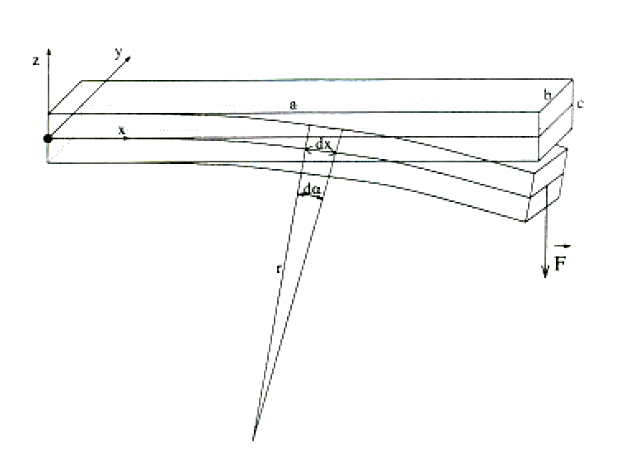
\includegraphics[width=0.6\textwidth]{../figures/balken_biegen.png}&
			\begin{align*}
			z=-\frac{12F}{Ebc^3}\left(\frac{ax^2}{2}-\frac{x^3}{6} \right)\\
			\Delta \varphi=\frac{\pi}{2}(2n+1)\hspace{0.5cm}\mbox{with }n=0,1,2,...\\
			y=\frac{\lambda}{4}(2n+1)\hspace{0.5cm}\mbox{with }n=0,1,2,...\\
			y(x)=A\cdot\left(5x^2-\frac{1}{6}x^3\right)+Bx+C\\
			E=\frac{12mg}{Abc^3}
			\end{align*}  
		\end{tabular}
	\end{table}
\end{frame}

\begin{frame}
	\frametitle{Double Exposure Hologram - Results}
  \begin{table}
  	\centering
  	\begin{tabular}[width=\textwidth]{m{3cm}m{3cm}m{3cm}}
  			\graTwoOneB[0.3]{Stab2R1-edit}{Stab1R2-edit}{Results for the Steel beam}&
  			\graTwoOneB[0.3]{Stab3R1-edit}{Stab2R2-edit}{Results for the Brass beam}&
  			\graTwoOneB[0.3]{Stab1R1-edit}{Stab3R2-edit}{Results for the Aluminium beam}
  	\end{tabular}
  \end{table}
	\begin{table}
		\begin{tabular}{c|ccc}
			Material&Steel&Brass&Aluminium\\\hline
			$E\,/\,\si{GPa}$&$196\pm5$&$104\pm3$&$68.5\pm1.6$\\
			$E_{lit}\,/\,\si{GPa}$\footfullcite{staats}&$195$&$100$&$72$
		\end{tabular}\\\scriptsize\ \\
		{\small Elastic Modules of Steel, Brass and Aluminium}
	\end{table}
	\pause
	\begin{itemize}
		\item Overexposure of Aluminium leads to difficult determination of the minima
		\pause
		\item Scaling and Evaluation with Gwyddion may be not enough accurate
	\end{itemize}
\end{frame}
\subsection{Real Time Hologram}
\frame{\tableofcontents[currentsubsection]}

\begin{frame}
	\frametitle{Real Time Hologram - Oscillations of an Aluminium Plate}	
	\begin{table}
		\centering
		\begin{tabular}{m{4.5cm}m{5.5cm}}
			
			\begin{align*}
				f_{m\nu}=\frac{x_{m\nu}^2h}{2\pi R^2}\sqrt{\frac{E}{12\rho(1-\mu^2)}}\\
				J_m(ix)\left[ J_{m-1}(x) - J_{m+1}(x)  \right]- \\iJ_m(x)\left[ J_{m-1}(ix) - J_{m+1}(ix)  \right] = 0
			\end{align*}
			\begin{itemize}
				\item Radius $R= (5.0\pm0.5)\,\mathrm{cm}$
				\item height $h=5\,\mathrm{mm}$
				\item Elastic Modulus $E =70\,\mathrm{GPa}$
				\item density $\rho = 2700\,\frac{\mathrm{kg}}{\mathrm{m^3}}$
				\item $\mu = 0.34$ 
			\end{itemize}
			&
			\gra[0.6]{bessel_2}{Bessel functions \footnotemark{}}\footnotetext{http://www.quanten.de/forum/showthread.php5?t=118}
		\end{tabular}
	\end{table}
\end{frame}
\begin{frame}
	\frametitle{Real Time Hologram - Set Up}
	\begin{figure}
		\centering
		\begin{overpic}[width=0.85\textwidth,tics=20]
			{../figures/aufbau3.png}
			\put(60,20){\footnotesize\textcolor{white}{Mirror 1}}
			\put(60,35){\footnotesize\textcolor{white}{Spatial Filter 1}}
			\put(34,50){\footnotesize\textcolor{white}{Mirror 2}}
			\put(40,47){\footnotesize\textcolor{white}{Spatial Filter 2}}
			\put(60,42){\footnotesize\textcolor{white}{Beam Splitter}}
			\put(65,57){\footnotesize\textcolor{white}{Laser}}
			\put(20,35){\footnotesize\textcolor{white}{Object}}
			\put(22,16){\footnotesize\textcolor{white}{Photo Plate}}
		\end{overpic}
	\end{figure}
\end{frame}

\begin{frame}
	\frametitle{Real Time Hologram - Experimental Procedure}
	\begin{itemize}
		\item Take a hologram of the aluminium plate in rest (same process as before)
		\item Stimulate the plate oscillations with a speaker
		\item Obstruct the reference beam
		\item Light the hologram with a pulsed object beam
		\item Go through the frequencies from about $100\,\si{Hz}$ to $6000\,\si{Hz}$ and search for resonance frequencies
	\end{itemize}
\end{frame}

\begin{frame}
	\frametitle{Real Time Hologram - Experimental Procedure}
	\begin{columns}
		\begin{column}{0.5\textwidth}
		\gra{oszi-inv}{Pulsing the Laser}%Set Up of the Michelson Interferometer}
		\end{column}
		\begin{column}{0.5\textwidth}
			\begin{itemize}
				\item Choose pulse duration short enough
				\item same frequency for both signals
				\item delay allows to choose the position of the pulse with respect to the speaker signal
			\end{itemize}
		\end{column}
	\end{columns}
\end{frame}



\begin{frame}
	\begin{table}[h]
		\centering
		\begin{tabular}{c|c|c}
			Mode 		& $x_{m\nu}$ & Calculated Frequency [Hz] 	 \\ \hline\hline
			$m=0,\nu=0$	&$3.19622$   &$5082$						\\ \hline
			$m=1,\nu=0$	& $4.61090$  & $10577$					\\ \hline
			$m=0,\nu=1$	& $6.30644$  & $19787$					\\ \hline
			$m=2,\nu=0$	& $5.90568$  & $17352$					\\ \hline
			$m=2,\nu=1$	& $9.19688$  & $42081$					\\ \hline
			$m=1,\nu=1$	& $7.79927$  & $30263$				     \\ \hline
			$m=3,\nu=0$	& $7.14353$  & $25388$                \\ \hline
			$m=3,\nu=1$	& $10.53670$ & $55235$
		\end{tabular} \vskip 0.2cm
		{Calculated Eigenfrequencies of the Aluminium plate}
	\end{table}	
\end{frame}
\begin{frame}
	\frametitle{Real Time Hologram - Results}
	\graTwoOneC{0.4}{0.2}{aluminium2_edit}{aluminium2_lit}{$f=(441.5\pm0.5)\,\si{Hz}$}
	\graTwoOneC{0.4}{0.2}{aluminium3_edit}{aluminium3_lit}{$f=(1059.0\pm1.0)\,\si{Hz}$}
\end{frame}
\begin{frame}
	\frametitle{Real Time Hologram - Results}
	\graTwoOneC{0.4}{0.2}{aluminium6_edit}{aluminium6_lit}{$f=(1716.0\pm1.0)\,\si{Hz}$}
	\graTwoOneC{0.4}{0.2}{aluminium7_edit}{aluminium7_lit}{$f=(2061.0\pm1.0)\,\si{Hz}$ *}
\end{frame}
\begin{frame}
	\frametitle{Real Time Hologram - Results}
	\graTwoOneC{0.4}{0.2}{aluminium9_edit}{aluminium9_lit}{$f=(2964\pm5)\,\si{Hz}$}
	\graTwoOneC{0.4}{0.2}{aluminium10_edit}{aluminium10_lit}{$f=(5383\pm5)\,\si{Hz}$}
\end{frame}

\begin{frame}
	\frametitle{Real Time Hologram - Results}
	\begin{columns}
		\begin{column}{0.6\textwidth}
			\begin{table}
				\centering
				\begin{tabular}{c|c|c|c}
					$m$ & $\nu$ 		& $f_{m\nu}\,/\,\si{Hz}$ 	& $f_{m\nu, \text{lit}}\,/\,\si{Hz}$\\ \hline\hline
					$0$&$0$	& $441.5\pm0.5$					& 448	\\ \hline
					$1$&$0$	& $1059\pm1.0$				& 983	\\ \hline
					$2$&$0$	& $1716\pm1.0$				& 1592	\\ \hline
					$2$&$1$	& $2061.0\pm1.0$ *				& 4090	\\ \hline
					$1$&$1$	& $2964\pm5$				& 2854 \\ \hline
					$3$&$1$	& $5383\pm5$				&-
				\end{tabular}\\\scriptsize\ \\\small
				{Results for the resonant frequencies\footnotemark}
			\end{table}		
		\end{column}
		\pause
%		\begin{column}{0.5\textwidth}
%			\begin{itemize}
%				\item Blabla
%			\end{itemize}
%		\end{column}
	\end{columns}
	\footnotetext{\fullcite{staats}}
\end{frame}

\begin{frame}
	\begin{columns}
	\begin{column}{0.5\textwidth}
		\gra{LinFitResFreq}{}
	\begin{itemize}
		\item Slope not significantly different from one
		\item Offset not significantly different from zero
		\item[]$\Rightarrow$ Validates our results
		\item Suggests underestimated statistical errors
	\end{itemize}
	\end{column}
	\begin{column}{0.5\textwidth}
		\gra{LinFitResFreq1}{}
	\begin{itemize}
		\item R-square-value: $0.9977$
		\item Supports linearity of the relation
		\item Confirms theoretical expectations
		\item[] \ 
	\end{itemize}
	\end{column}
	\end{columns}
\end{frame}

\subsection{Fourier Interferometry}
\frame{\tableofcontents[currentsubsection]}
\begin{frame}
	\frametitle{Fourier Optics - Huygen's Principle and Fraunhofer Diffraction}
	\gra[0.6]{Huygen}{Propagation of Waves based on Huygen's Principle \footnote{http://web.mit.edu/viz/EM/visualizations/coursenotes/modules/guide14.pdf}}
		Fresnel-Kirchhoff-Integral Formula:
		\begin{align}
		U(x_0) &= \frac{1}{\lambda L} C \mathscr{F}{g(x, y)}    = \frac{1}{\lambda L} C   \int\limits_{-\infty}^{\infty}  g(x,y)e^{-ikx}dx    &  C  \cdot C^* &= 1       
		\end{align}
		
		Intensity Distribution in the Far field:
		\begin{align}
		I=|U(x_0)|^2=\left| \int\limits_{-\infty}^{\infty} g(x,y)e^{-ikx}dx \right|^2
		\end{align}
\end{frame}

\begin{frame}
	\frametitle{Fourier Transform of a Single Slit}
\gra[0.8]{Einzelspalt}{Fourier optics for a single slit \footnote{https://www.chem.purdue.edu/courses/chm621/text/ft/basiset/rect/rectangle.gif}}
\end{frame}


\begin{frame}
	\frametitle{Convolution Theorem}
		\begin{table}
			\centering
			\begin{tabular}[width=\textwidth]{m{6cm}m{4cm}}
				
				
			$	(f*g)(t)=\int\limits_{-\infty}^{\infty} f(\tau)\cdot g(t-\tau) d\tau $ \newline
			$	\mathscr{F}(f*g)=const. \mathscr{F}(f)\cdot \mathscr{F}(g) $
				&
				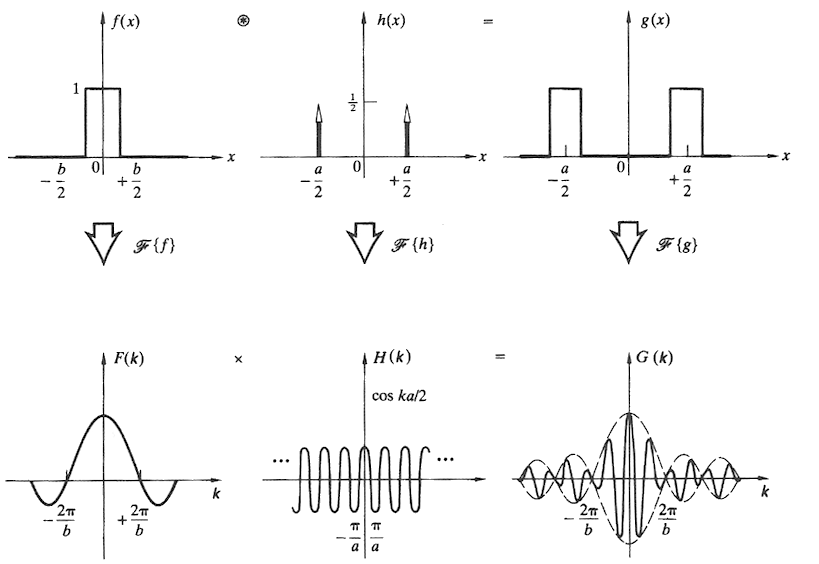
\includegraphics[width=0.4\textwidth]{../figures/Convolution.png}\\
			
			\end{tabular}
		\end{table}
		\footnotetext{http://www4.uwsp.edu/physastr/kmenning/images/Hecht4.11.F.31.png}
\end{frame}
\begin{frame}
	\frametitle{Cross- and Autocorrelation}
		\begin{table}
			\centering
			\begin{tabular}[width=\textwidth]{m{6cm}m{4cm}}
				
				
			\textbf{Cross-Correlation} describes the similarity of two functions dependent on the displacement of one relative to another:
			$ (f*g)(t)=\int\limits_{-\infty}^{\infty} f(\tau)\cdot g(t+\tau) d\tau \label{corr} $
			\textbf{Auto-Correlation} describes the self-similarity of a function with a displaced version of itself
				&
		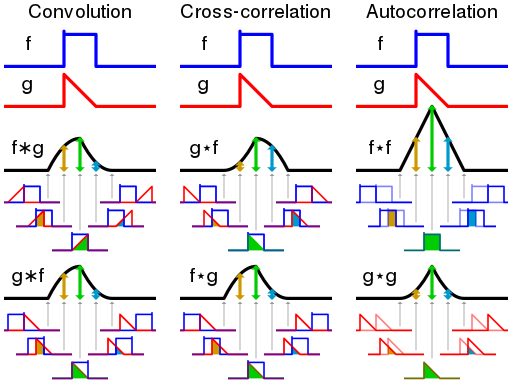
\includegraphics[width=0.4\textwidth]{../figures/correlation.png}\footnotetext{By Cmglee - Own work, CC BY-SA 3.0, https://commons.wikimedia.org/w/index.php?curid=20206883}\\
				
			\end{tabular}
		\end{table}
\end{frame}

\begin{frame}
	\frametitle{4f-Correlator}
	\gra[0.8]{Correlator}{4f-Correlator (with no mask in the transform plane)\footnote{http://www4.uwsp.edu/physastr/kmenning/images/Hecht4.11.F.26.png}} 
\end{frame}

\begin{frame}
	\frametitle{Fourier Interferometry - Experimental Set Up}
   \gra[0.72]{Versuchsaufbau_4}{Experimental set-up for the cross-correlation measurement  \footfullcite{Bamberger}}
\end{frame}
\begin{frame}
	\frametitle{Fourier Interferometry - Experimental Set Up}
	\gra[0.8]{aufbau4}{Experimental set-up for the cross-correlation measurement}
\end{frame}

\begin{frame}
	\frametitle{Fourier Interferometry - Results}
\begin{table}
	\centering
	\begin{tabular}{m{5cm}m{5cm}}
	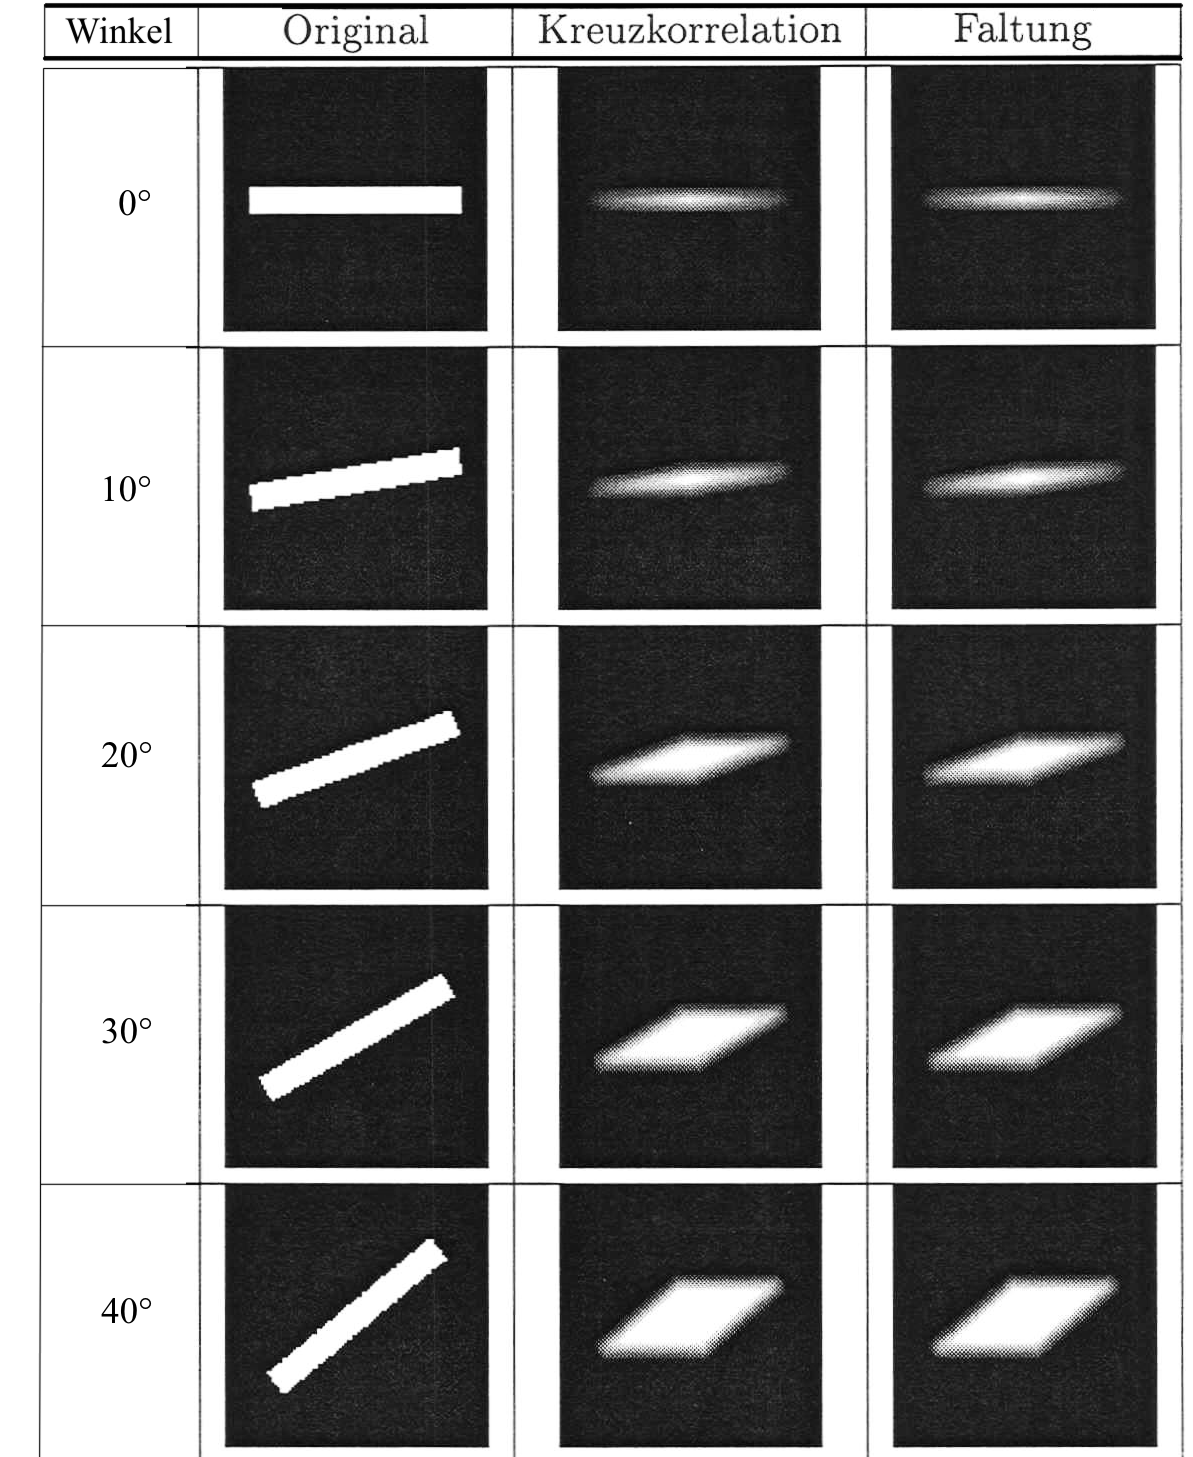
\includegraphics[width=0.4\textwidth]{../figures/Korrelation_Spalt1.png}	

	&
	\begin{minipage}{0.6\textwidth}
		\centering
		\begin{overpic}[width=0.3\textwidth,tics=10]{../figures/fourier-0-2-edit.png}
			\put(10,85){\Large\textcolor{white}{$\alpha=0\degree$}}
		\end{overpic}
		\begin{overpic}[width=0.3\textwidth,tics=10]{../figures/fourier-15-2-edit.png}
			\put(10,85){\Large\textcolor{white}{$\alpha=15\degree$}}
		\end{overpic}\\
		\vspace{0.2 cm}
		\begin{overpic}[width=0.3\textwidth,tics=10]{../figures/fourier-30-2-edit.png}
			\put(10,85){\Large\textcolor{white}{$\alpha=30\degree$}}
		\end{overpic}
		\begin{overpic}[width=0.3\textwidth,tics=10]{../figures/fourier-45-2-edit.png}
			\put(10,85){\Large\textcolor{white}{$\alpha=45\degree$}}
		\end{overpic}\\
	\end{minipage}
    \end{tabular}
\end{table}
\footfullcite{anleitung}
\end{frame}

\begin{frame}
	\frametitle{Fourier Interferometry - Results}
	\begin{table}
		\centering
		\begin{tabular}{m{5cm}m{5cm}}
			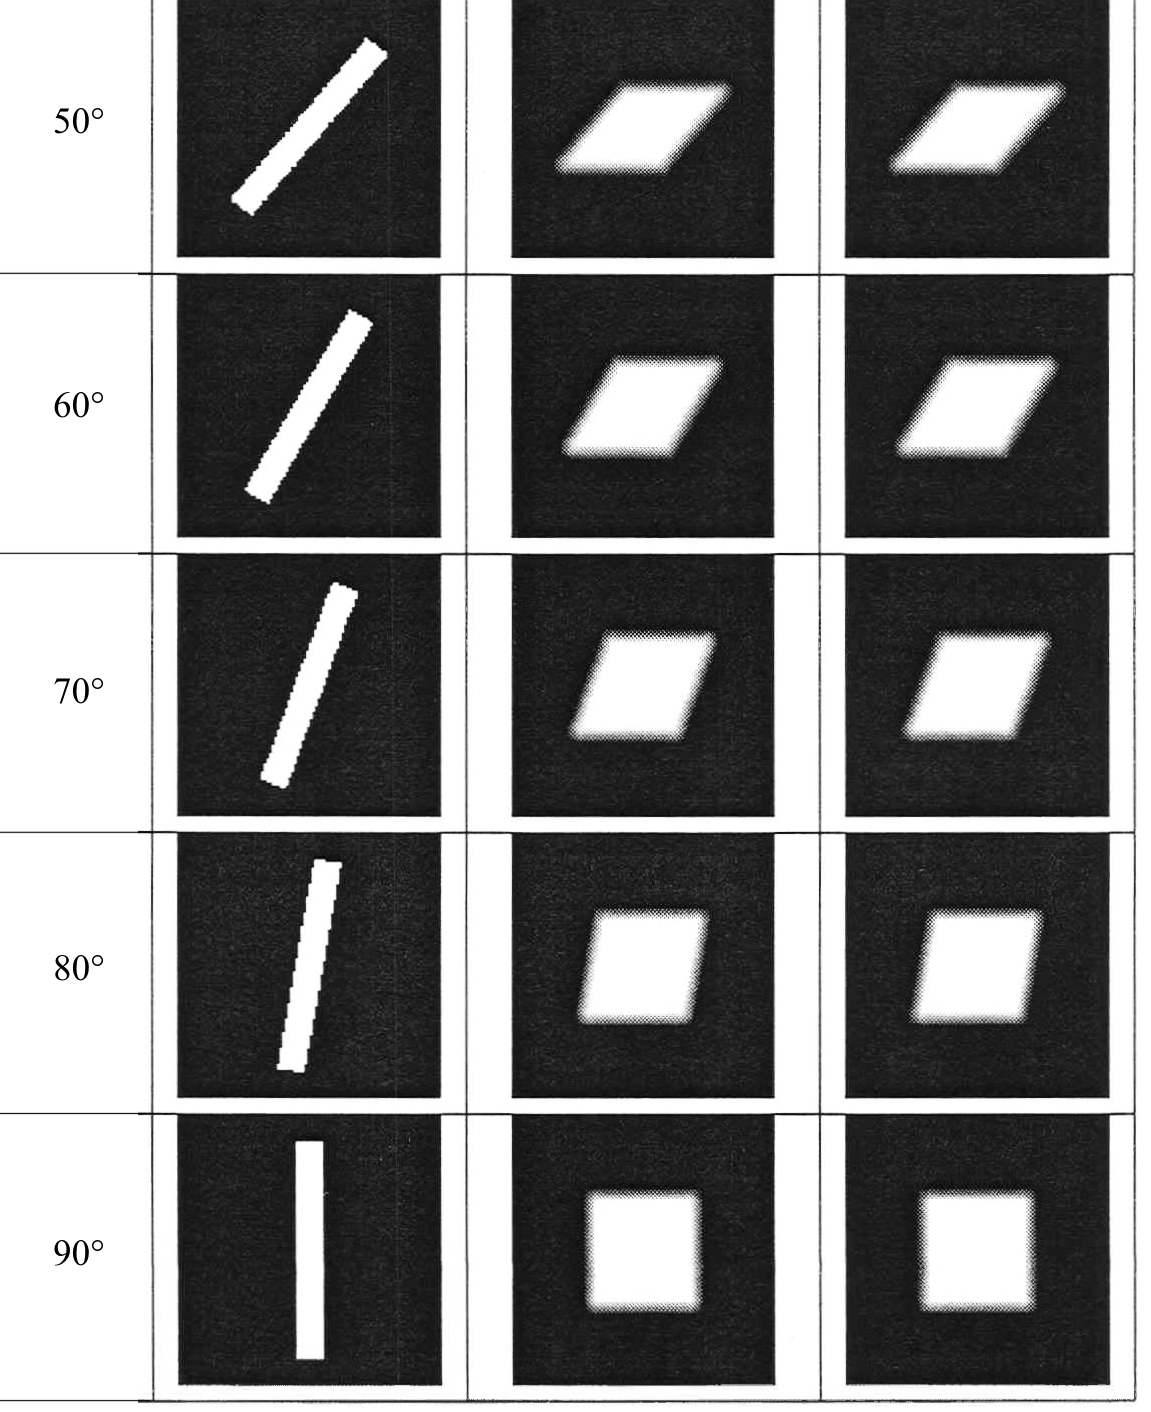
\includegraphics[width=0.4\textwidth]{../figures/Korrelation_Spalt2.png}	
			
			&
			\begin{minipage}{0.6\textwidth}
				\centering
				\begin{overpic}[width=0.3\textwidth,tics=10]{../figures/fourier-60-2-edit.png}
					\put(10,85){\Large\textcolor{white}{$\alpha=60\degree$}}
				\end{overpic}
				\begin{overpic}[width=0.3\textwidth,tics=10]{../figures/fourier-75-2-edit.png}
					\put(10,85){\Large\textcolor{white}{$\alpha=75\degree$}}
				\end{overpic}\\
				\vspace{0.2 cm}
				\begin{overpic}[width=0.3\textwidth,tics=10]{../figures/fourier-90-2-edit.png}
					\put(10,85){\Large\textcolor{white}{$\alpha=90\degree$}}
				\end{overpic}\\
			\end{minipage}
		\end{tabular}
	\end{table}
\footfullcite{anleitung}
\end{frame}

\begin{frame}
	\frametitle{Fourier Interferometry - Results}
	\begin{table}
		\centering
		\begin{tabular}{m{5cm}m{5cm}}
			\begin{figure}
				\centering
				\begin{overpic}[width=0.135\textwidth,tics=10]
					{../figures/fourier-0-2-edit.png}
					\put(10,80){\textcolor{white}{$\alpha=0\degree$}}
				\end{overpic}
				\begin{overpic}[width=0.135\textwidth,tics=10]
					{../figures/fourier-15-2-edit.png}
					\put(10,80){\textcolor{white}{$\alpha=15\degree$}}
				\end{overpic}
				\begin{overpic}[width=0.135\textwidth,tics=10]
					{../figures/fourier-30-2-edit.png}
					\put(10,80){\textcolor{white}{$\alpha=30\degree$}}
				\end{overpic}\\
				\vspace{0.1 cm}
				\begin{overpic}[width=0.135\textwidth,tics=10]
					{../figures/fourier-45-2-edit.png}
					\put(10,80){\textcolor{white}{$\alpha=45\degree$}}
				\end{overpic}
				\begin{overpic}[width=0.135\textwidth,tics=10]
					{../figures/fourier-60-2-edit.png}
					\put(10,80){\textcolor{white}{$\alpha=60\degree$}}
				\end{overpic}
				\begin{overpic}[width=0.135\textwidth,tics=10]
					{../figures/fourier-75-2-edit.png}
					\put(10,80){\textcolor{white}{$\alpha=75\degree$}}
				\end{overpic}\\
				
				\vspace{0.1 cm}
				
				\begin{overpic}[width=0.135\textwidth,tics=10]
					{../figures/fourier-90-2-edit.png}
					\put(10,80){\textcolor{white}{$\alpha=90\degree$}}
				\end{overpic}
			\end{figure}
			&\pause
			\begin{itemize}
				\item Cross Correlation can be seen with bare eyes\pause
				\item Difficult to take pictures\pause
				\item Very dark because of bad bleaching\pause
				\item Difficult to find good focus settings
			\end{itemize}
		\end{tabular}
	\end{table}
\end{frame}
%\begin{frame}
%\frametitle{Fourier Interferometry - Results}
%\begin{figure}
%	
%	\begin{overpic}[width=0.3\textwidth,tics=10]
%		{../figures/fourier-60-2-edit.png}
%		\put(10,85){\Large\textcolor{white}{$\alpha=60\degree$}}
%	\end{overpic}
%	\begin{overpic}[width=0.3\textwidth,tics=10]
%		{../figures/fourier-75-2-edit.png}
%		\put(10,85){\Large\textcolor{white}{$\alpha=75\degree$}}
%	\end{overpic}\\
%	
%	\vspace{0.2 cm}
%	
%	\begin{overpic}[width=0.3\textwidth,tics=10]
%		{../figures/fourier-90-2-edit.png}
%		\put(10,85){\Large\textcolor{white}{$\alpha=90\degree$}}
%	\end{overpic}
%
%\end{figure}
%\end{frame}
%\begin{frame}
%	\frametitle{Fourier Interferometry - Comparison with Theoretical Results}
%\graTwoOne[0.4]{Korrelation_Spalt1}{Korrelation_Spalt2}{Theoretical Predictions}
%\end{frame}

\section{Summary and Discussion}
\frame{\tableofcontents[currentsection]}
\begin{frame}
	\frametitle{Summary of the Results}
	\begin{columns}
		\begin{column}{0.6\textwidth}
			\begin{table}[h]
				\begin{tabular}{c|ccc}
					Material&Steel&Brass&Aluminium\\\hline
					$E\,/\,\si{GPa}$&$196\pm5$&$104\pm3$&$68.5\pm1.6$\\
					$E_{lit}\,/\,\si{GPa}$&$195$&$100$&$72$
				\end{tabular}\\\scriptsize\ \\
				{\small Elastic Modules of Steel, Brass and Aluminium}
			\end{table}
			\begin{table}[h]
				\centering
				\begin{tabular}{c|c|c|c}
					$m$ & $\nu$ 		& $f_{m\nu}\,/\,\si{Hz}$ 	& $f_{m\nu, \text{lit}}\,/\,\si{Hz}$\\ \hline\hline
					$0$&$0$	& $441.5\pm0.5$					& 448	\\ \hline
					$1$&$0$	& $1059\pm1.0$				& 983	\\ \hline
					$2$&$0$	& $1716\pm1.0$				& 1592	\\ \hline
					$2$&$1$	& $2061.0\pm1.0$				& 4090	\\ \hline
					$1$&$1$	& $2964\pm5$				& 2854 \\ \hline
					$3$&$1$	& $5383\pm5$				&-
				\end{tabular}\\\scriptsize\ \\\small
				{Results for the resonant frequencies}
			\end{table}		
		\end{column}
		%\pause
		\begin{column}{0.3\textwidth}
			\begin{figure}[h]
				\centering
				\begin{overpic}[width=0.27\textwidth,tics=10]
					{../figures/fourier-0-2-edit.png}
					\put(10,80){\textcolor{white}{$\alpha=0\degree$}}
				\end{overpic}
				\begin{overpic}[width=0.27\textwidth,tics=10]
					{../figures/fourier-15-2-edit.png}
					\put(10,80){\textcolor{white}{$\alpha=15\degree$}}
				\end{overpic}
				\begin{overpic}[width=0.27\textwidth,tics=10]
					{../figures/fourier-30-2-edit.png}
					\put(10,80){\textcolor{white}{$\alpha=30\degree$}}
				\end{overpic}\\
				\vspace{0.1 cm}
				\begin{overpic}[width=0.27\textwidth,tics=10]
					{../figures/fourier-45-2-edit.png}
					\put(10,80){\textcolor{white}{$\alpha=45\degree$}}
				\end{overpic}
				\begin{overpic}[width=0.27\textwidth,tics=10]
					{../figures/fourier-60-2-edit.png}
					\put(10,80){\textcolor{white}{$\alpha=60\degree$}}
				\end{overpic}
				\begin{overpic}[width=0.27\textwidth,tics=10]
					{../figures/fourier-75-2-edit.png}
					\put(10,80){\textcolor{white}{$\alpha=75\degree$}}
				\end{overpic}\\
				
				\vspace{0.1 cm}
				
				\begin{overpic}[width=0.27\textwidth,tics=10]
					{../figures/fourier-90-2-edit.png}
					\put(10,80){\textcolor{white}{$\alpha=90\degree$}}
				\end{overpic}
			\end{figure}
		\end{column}
		\Footnotetext{ }{Literaturwerte aus \fullcite{staats}}
	\end{columns}
	
\end{frame}

\begin{frame}
	\LARGE{Fragen?}
\end{frame}


\begin{frame}
	\frametitle{Types of Holography}
	\gra[0.5]{Reflex_Transmissions_Hologram}{Comparison of Reflection and Transmission Hologram  \footfullcite{staats}}
\end{frame}

\begin{frame}
	\frametitle{Spatial Filter}
	\gra[0.8]{SpatialFilter}{Set-Up of a Spatial Filter }
\end{frame}

\begin{frame}
	\frametitle{Hologram of an object point}
	\gra[0.5]{obj2}{Blackness of a photo plate for two and four object points respectively \footfullcite{staats}}
\end{frame}

\begin{frame}
	\frametitle{Pockels Cell}
	\begin{itemize}
	\item change of the refracting properties of an opitical medium induced by an electric field
	\item birefringence: refractive index depending on the polarization of light and/or the propagation direction of light
	\end{itemize}
\end{frame}

\end{document}